\documentclass{scrartcl}
\usepackage[margin=3cm]{geometry}
\usepackage{amsmath}
\usepackage{amssymb}
\usepackage{amsthm}
\usepackage{blindtext}
\usepackage{datetime}
\usepackage{fontspec}
\usepackage{float}
\usepackage{graphicx}
\usepackage{kotex}
\usepackage[lighttt]{lmodern}
\usepackage{listings}
\usepackage{mathrsfs}
\usepackage{mathtools}
\usepackage{pgf,tikz,pgfplots}

\pgfplotsset{compat=1.15}
\usetikzlibrary{arrows}
\newtheorem{theorem}{Theorem}

\lstset{
  numbers=none, frame=single, showspaces=false,
  showstringspaces=false, showtabs=false, breaklines=true, showlines=true,
  breakatwhitespace=true, basicstyle=\ttfamily, keywordstyle=\bfseries, basewidth=0.5em
}

\setmainhangulfont{Noto Serif CJK KR}[
  UprightFont=* Light, BoldFont=* Bold,
  Script=Hangul, Language=Korean, AutoFakeSlant,
]
\setsanshangulfont{Noto Sans CJK KR}[
  UprightFont=* DemiLight, BoldFont=* Medium,
  Script=Hangul, Language=Korean
]
\setmathhangulfont{Noto Sans CJK KR}[
  SizeFeatures={
    {Size=-6,  Font=* Medium},
    {Size=6-9, Font=*},
    {Size=9-,  Font=* DemiLight},
  },
  Script=Hangul, Language=Korean
]
\title{디지털시스템설계 Lab 4}
\author{손량(20220323)}
\date{Last compiled on: \today, \currenttime}

\newcommand{\un}[1]{\ensuremath{\ \mathrm{#1}}}

\begin{document}
\maketitle

\section{개요}
이번 lab 4에서는 이진수의 연산에 사용되는 반가산기와 전가산기를 구현하고, 이들을 통해 덧셈, 뺄셈, 곱셈 회로를 구현해 본다.

\section{이론적 배경}
\subsection{반가산기와 전가산기}
반가산기는 1-bit 이진수를 두 개 입력받아 더한 값과 carry out을 출력하는 소자이다.
전가산기는 1-bit 이진수와 이전 가산기의 carry in을 입력받아 합, carry out을 출력한다.
사실상 세 개의 1-bit 이진수를 입력받아 더한 2-bit 결과를 줄력한다고도 할 수 있다.

\subsection{\(N\)-bit Ripple Carry Adder/Subtractor}
\(N\)-bit ripple carry adder는 \(N\)-bit 이진수 두 개를 더한 \(N\)-bit 결과와 carry out을 출력한다.
리플 가산기는 \(N\)개의 전가산기를 차례차례 이어서 구현한다.
각 전가산기는 각 자리의 연산을 수행하고, 자신의 carry out을 자신보다 한 단계 상위 비트를 연산하는 전가산기의 carry in에 전달한다.
이러한 설계에서, carry out 신호는 이름이 의미하는 바와 같이 파도처럼 전가산기 하나씩 전파된다.

\(N\)비트 리플 가산기를 사용하면 뺄셈도 처리할 수 있다.
2의 보수 표현법을 사용하면 다음이 성립하고,
\begin{align*}
  A - B = A + (-B) = A + B' + 1
\end{align*}
가장 하위 비트를 연산하는 전가산기의 carry in에 1을 입력하고, \(B\)의 모든 비트를 반전시켜 전가산기에 입력하면 된다.

\subsection{Binary Multiplier}
\(M\)비트 이진수 \(a_{M - 1} a_{M - 2} \dots a_0\)과 \(N\)비트 이진수 \(b_{N - 1} b_{N - 2} \dots b_0\)을 곱한다고 하자.
이때 다음과 같이 쓸 수 있다.
\begin{align*}
  &a_{M - 1} a_{M - 2} \dots a_0 \times b_{N - 1} b_{N - 2} \dots b_0 \\
  &= 2^0 b_0 (a_{M - 1} a_{M - 2} \dots a_0) + 2^1 b_1 (a_{M - 1} a_{M - 2} \dots a_0) + \dots + 2^{N - 1} b_{N - 1} (a_{M - 1} a_{M - 2} \dots a_0) \\
  &= \sum^{N - 1}_{k = 0} 2^k b_k (a_{M - 1} a_{M - 2} \dots a_0)
\end{align*}
AND 게이트를 사용하여 1-bit \(b_0, b_1, \dots, b_{N - 1}\)과 \(a_{M - 1} a_{M - 2} \dots a_0\)의 곱셈을 구현하고 \(M\)-bit adder로 중간 결과를 더하도록 구현할 수 있다.

\section{실험 준비}
\subsection{반가산기}
반가산기의 진리표는 다음과 같다.
\begin{table}[H]
  \centering
  \begin{tabular}{ll|ll}
    \hline
    \(A\) & \(B\) & \(S\) & \(C\) \\
    \hline
    0 & 0 & 0 & 0 \\
    0 & 1 & 1 & 0 \\
    1 & 0 & 1 & 0 \\
    1 & 1 & 0 & 1 \\
    \hline
  \end{tabular}
\end{table}
이 진리표를 는리식으로 나타내면 다음과 같다.
\begin{align*}
  S &= A' B + AB' = A \oplus B \\
  C &= AB
\end{align*}
회로로 나타내면 다음과 같다.
\begin{figure}[H]
  \centering
  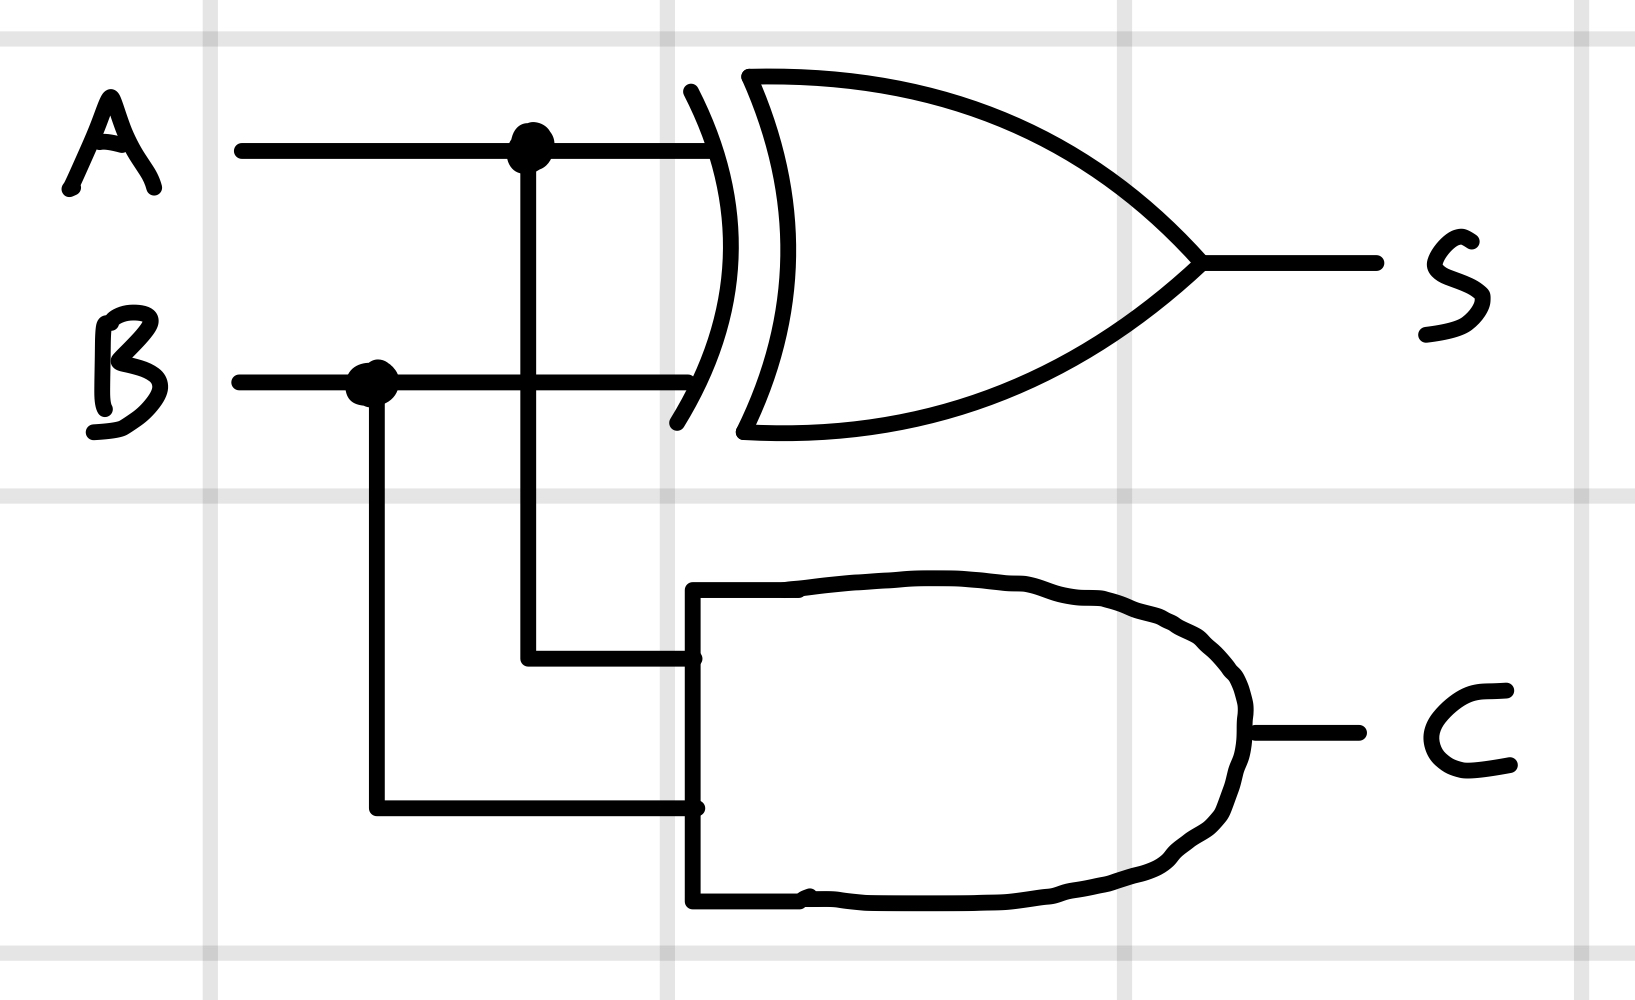
\includegraphics[width=0.3\linewidth]{half-adder.jpeg}
\end{figure}

\subsection{전가산기}
전가산기의 진리표는 다음과 같다.
\begin{table}[H]
  \centering
  \begin{tabular}{ccc|cc}
    \hline
    \(A\) & \(B\) & \(C_\text{in}\) & \(S\) & \(C_\text{out}\) \\
    \hline
    0 & 0 & 0 & 0 & 0 \\
    0 & 0 & 1 & 1 & 0 \\
    0 & 1 & 0 & 1 & 0 \\
    0 & 1 & 1 & 0 & 1 \\
    1 & 0 & 0 & 1 & 0 \\
    1 & 0 & 1 & 0 & 1 \\
    1 & 1 & 0 & 0 & 1 \\
    1 & 1 & 1 & 1 & 1 \\
    \hline
  \end{tabular}
\end{table}
는리식으로 쓰면
\begin{align*}
  S &= A \oplus B \oplus C_\text{in} \\
  C_\text{out} &= AB + BC_\text{in} + AC_\text{in} = AB + A' BC_\text{in} + AB' C_\text{in} = AB + (A \oplus B) C_\text{in}
\end{align*}
\(A\)와 \(B\)를 반가산기로 연산했을 때 합을 \(S_{AB} := A \oplus B\), carry out을 \(C_{AB} := AB\)라고 할 때
\begin{align*}
  S &= S_{AB} \oplus C_\text{in} \\
  C_\text{out} &= C_{AB} + S_{AB} C_\text{in}
\end{align*}
이 식을 사용하면 반가산기를 통해 다옴과 같이 회로도를 그릴 수 있다.\footnote{여기서 전선이 교차하는 점은 연결점이 아니다.}
\begin{figure}[H]
  \centering
  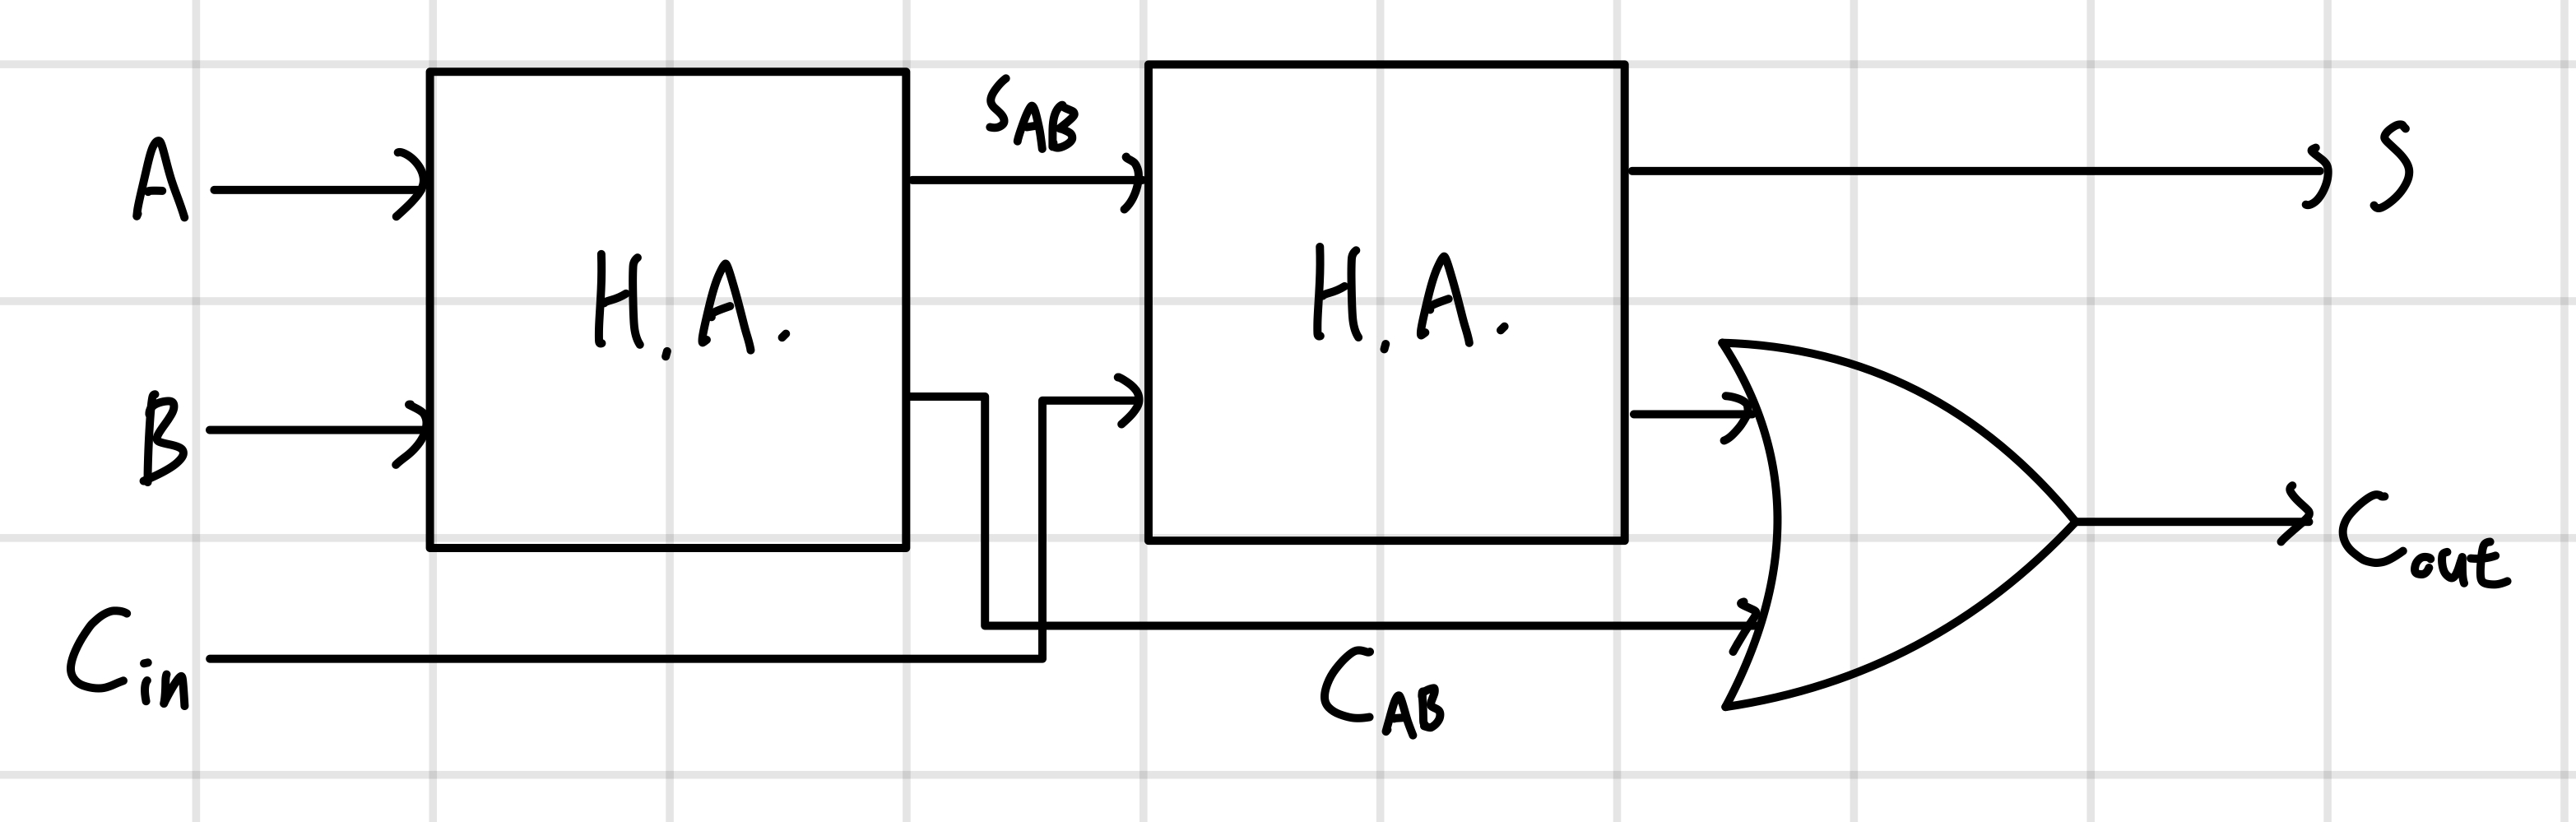
\includegraphics[width=0.75\linewidth]{full-adder.jpeg}
\end{figure}

\subsection{5-bit 리플 가산기/감산기}
5-bit 이진수 \(A = A_4 A_3 A_2 A_1 A_0, B = B_4 B_3 B_2 B_1 B_0\)을 연산한다고 하자.
5개의 전가산기를 활용하여, 각 전가산기마다 입력된 숫자의 각 비트를 연산하도록 설계할 수 있다.
LSB를 연산하는 전가산기의 carry in에는 0을 입력하고, 각 전가산기의 carry out을 한 단계 상위 비트를 연산하는 전가산기의 carry in에 연결하면 된다.
\begin{figure}[H]
  \centering
  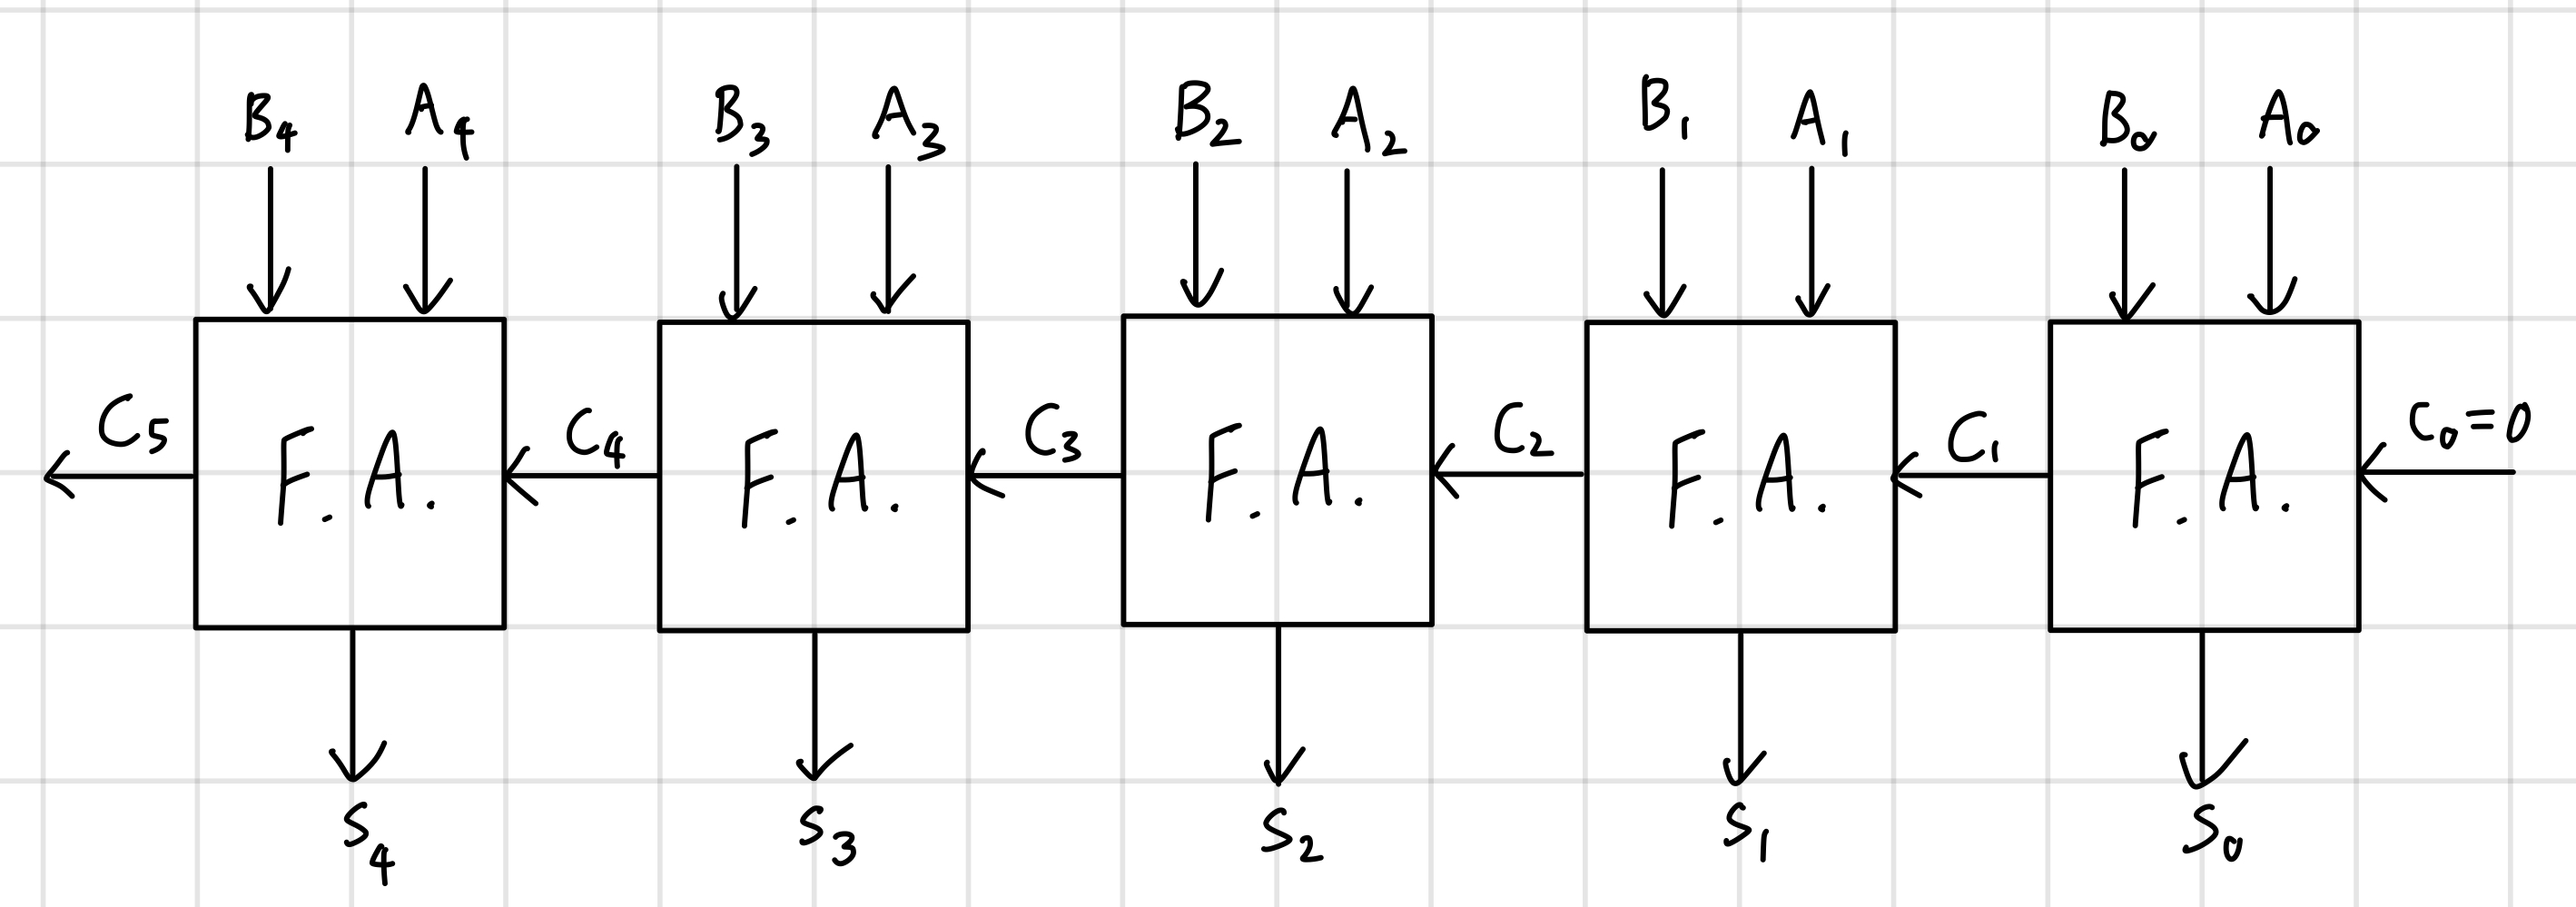
\includegraphics[width=0.8\linewidth]{ripple-carry-adder.jpeg}
\end{figure}
음수를 2의 보수로 표현한다면 \(A - B = A + (-B) = A + B' + 1\)이고, 2의 보수 체계에는 unsigened integer인 것처럼 생각하고 덧셈을 진행할 수 있으므로 앞선 덧셈을 계산하는 회로에서 \(B_0, B_1, \dots, B_4\)를 반전한 다음, \(C_0 = 1\)을 입력하면 \(A + B' + 1\), 즉 \(A - B\)를 계산할 수 있다.
회로도는 다음과 같다.
\begin{figure}[H]
  \centering
  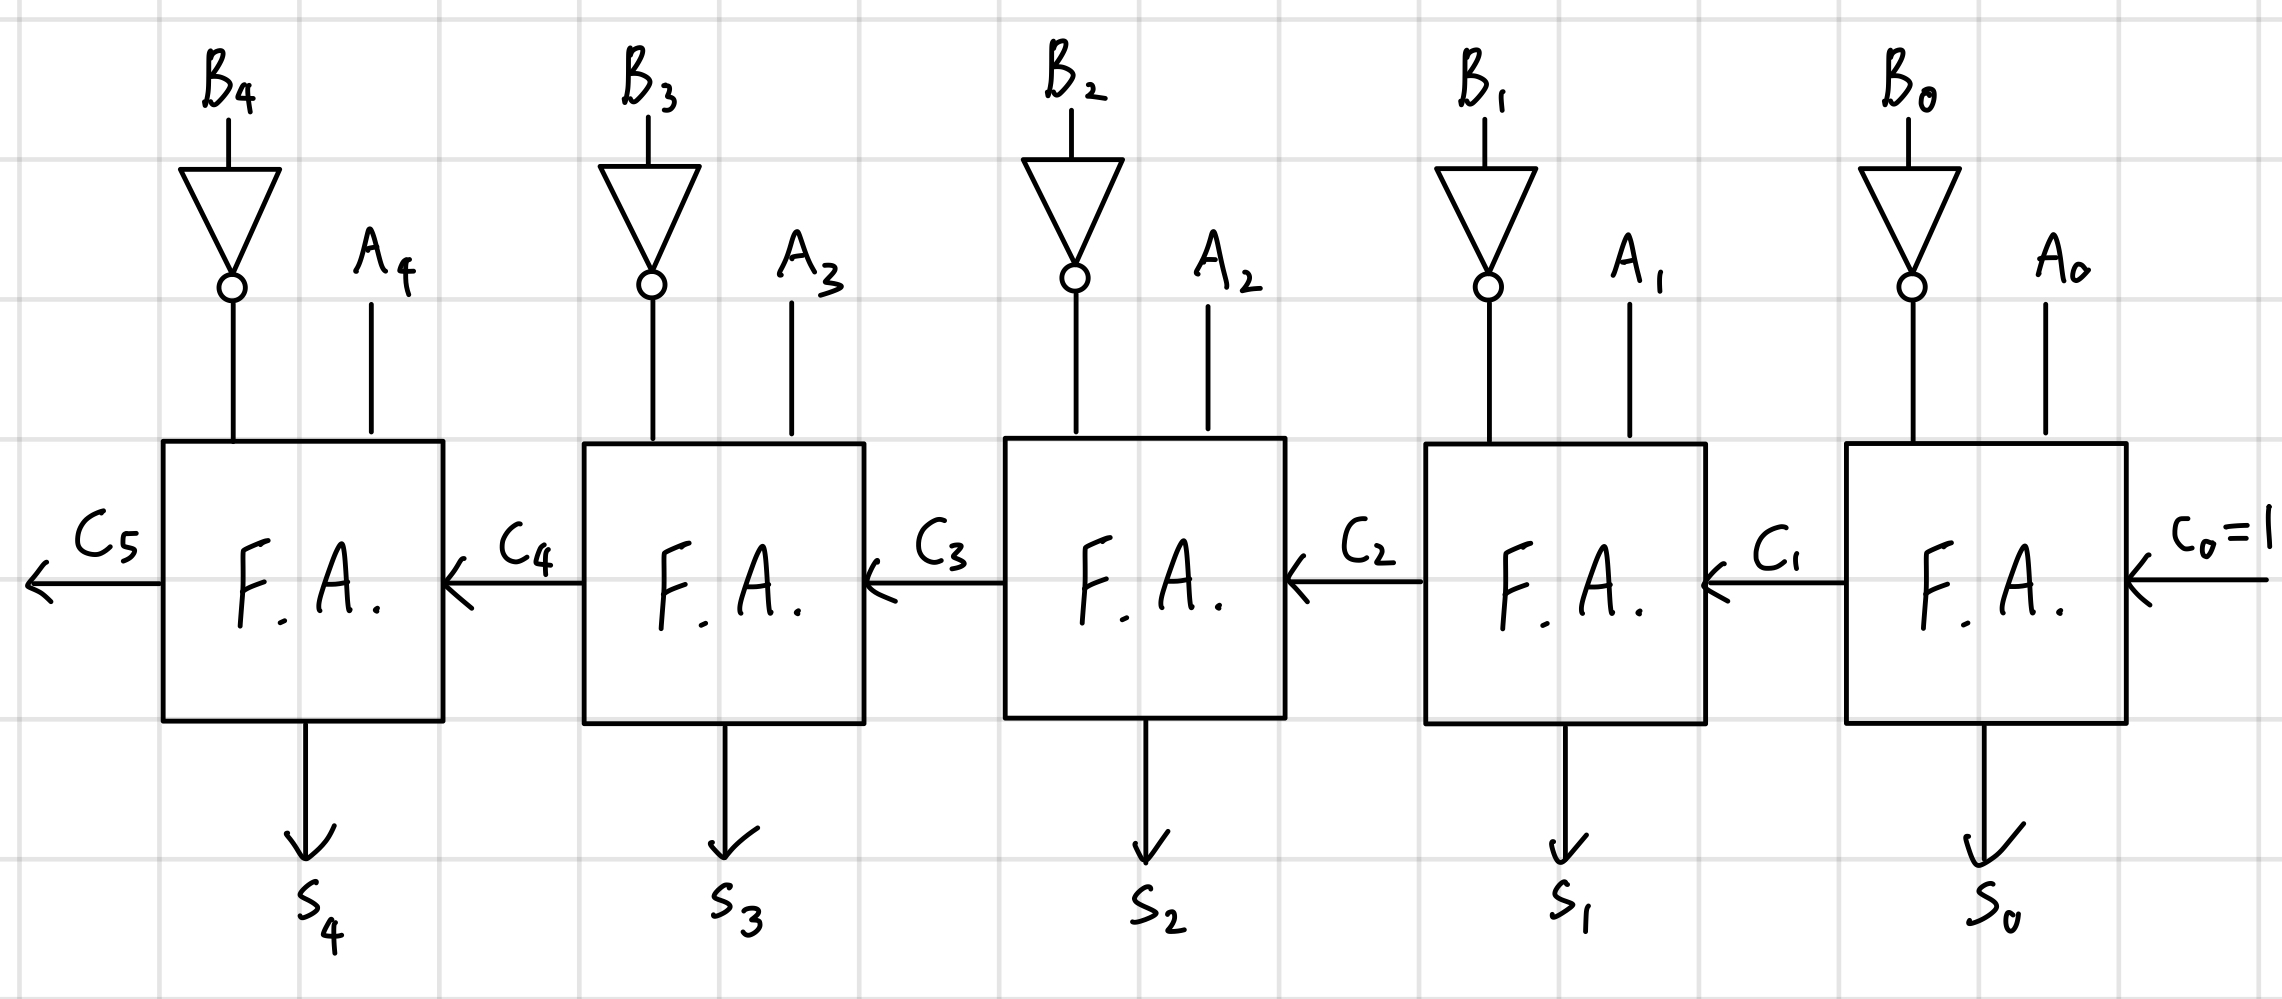
\includegraphics[width=0.8\linewidth]{ripple-carry-subtractor.jpeg}
\end{figure}

\subsection{5-by-3 Binary Multiplier}
5-bit 이진수 \(A = A_4 A_3 A_2 A_1 A_0\)과 \(B = B_2 B_1 B_0\)을 곱해 8-bit 이진수 \(C = C_7 C_6 \dots C_0\)을 얻는다고 하자.
\(A\)와 \(B_0, B_1, B_2\) 사이의 곱셈은 AND 게이트를 사용해서 계산할 수 있고, 이렇게 구한 부분 결과들을 5-bit 리플 가산기를 활용하여 더하면 곱셈 결과를 얻는다.
회로도로 나타내면 다음과 같다.
\begin{figure}[H]
  \centering
  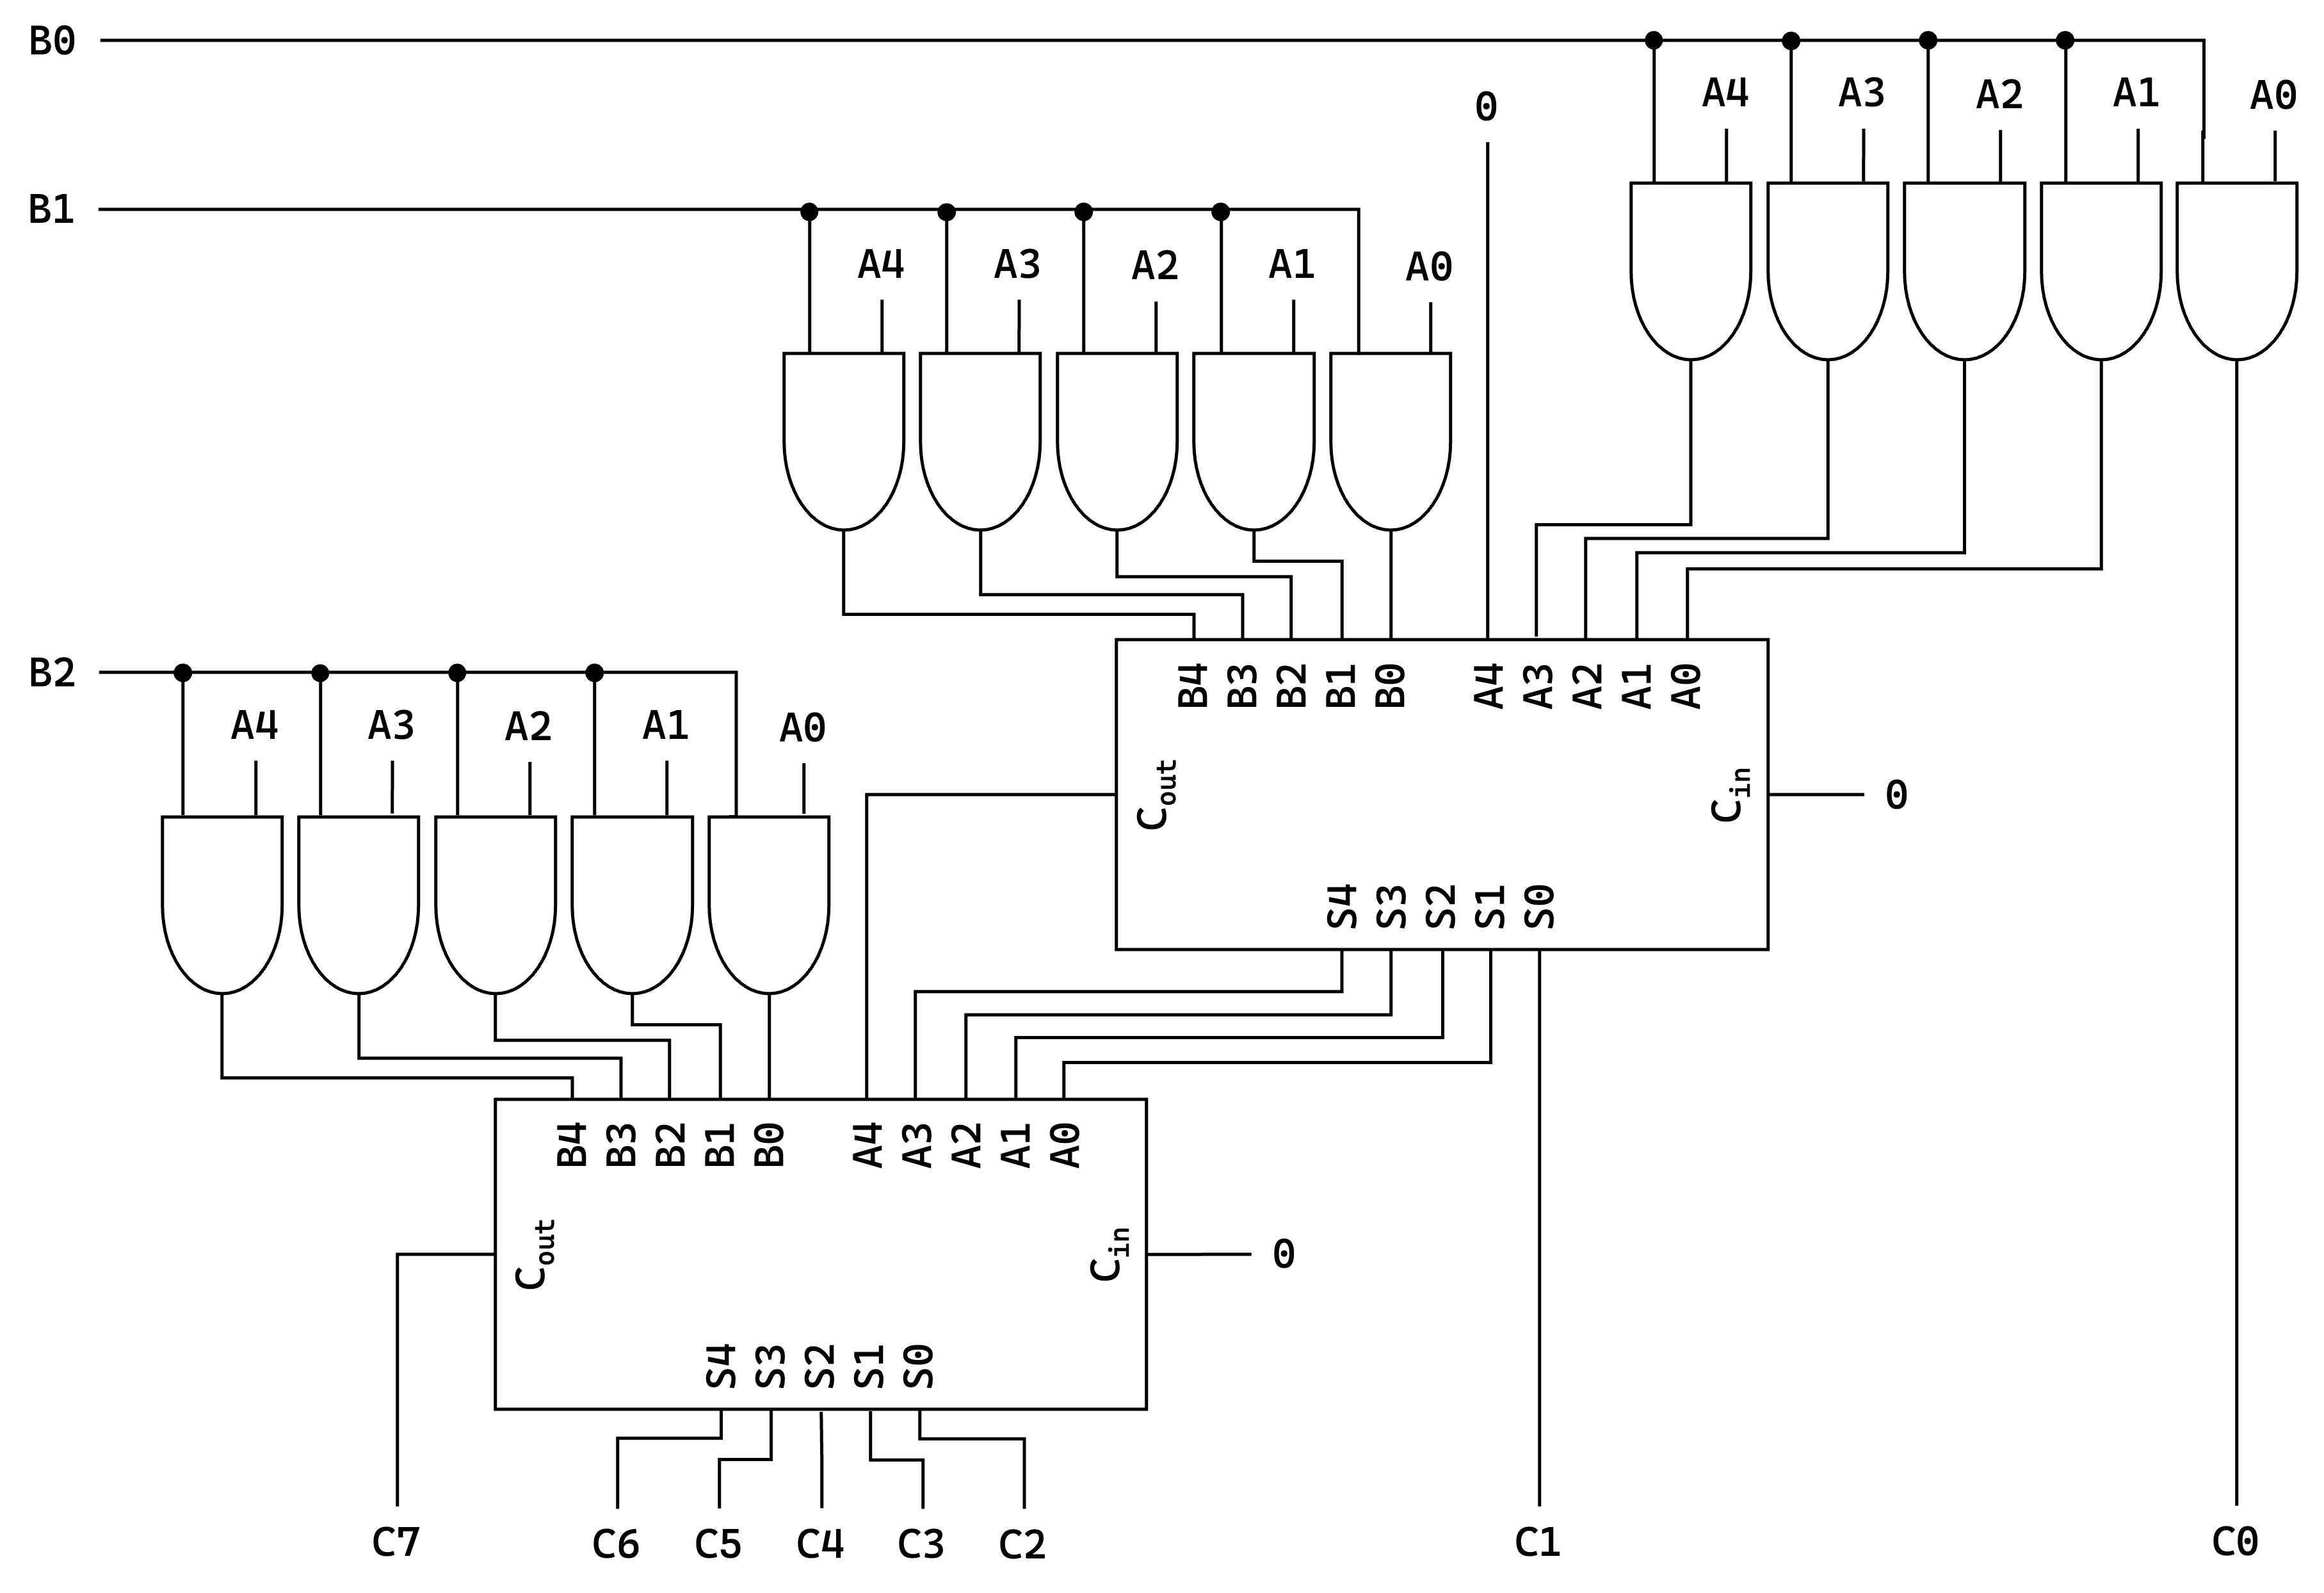
\includegraphics[width=0.9\linewidth]{multiplier.png}
\end{figure}

\section{실험 결과}
\subsection{\texttt{lab4\_1.v} -- 반가산기, 전가산기}
반가산기의 회로도는 다음과 같다.
\begin{figure}[H]
  \centering
  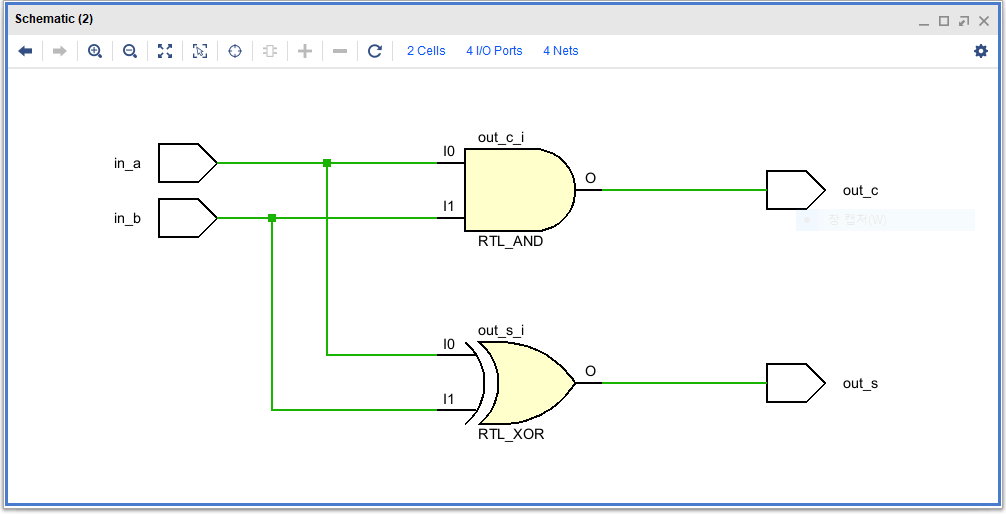
\includegraphics[width=0.9\linewidth]{lab4_1_half_schematic.png}
\end{figure}
전가산기의 회로도는 다음과 같다.
\begin{figure}[H]
  \centering
  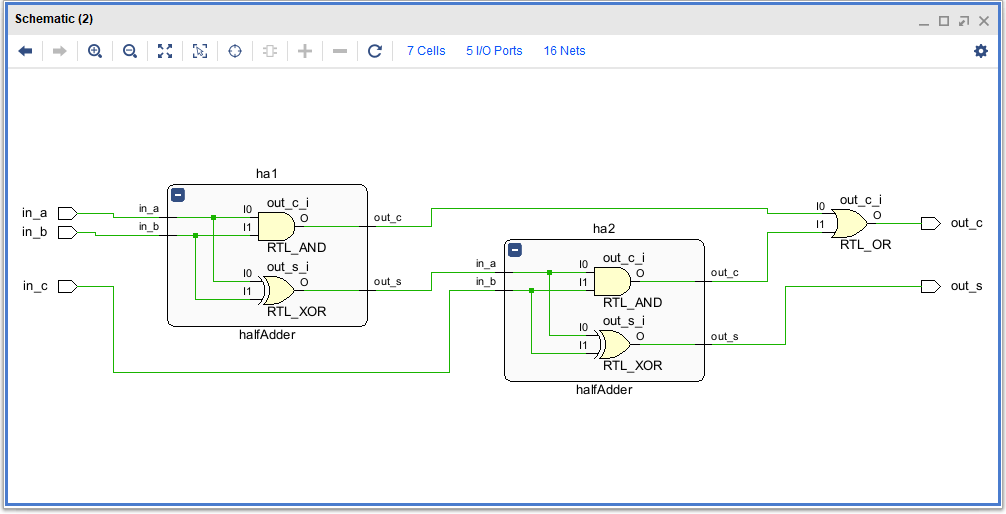
\includegraphics[width=0.9\linewidth]{lab4_1_full_schematic.png}
\end{figure}

\subsection{\texttt{lab4\_2.v} -- 5-bit 리플 가산기}
회로도는 다음과 같다.
\begin{figure}[H]
  \centering
  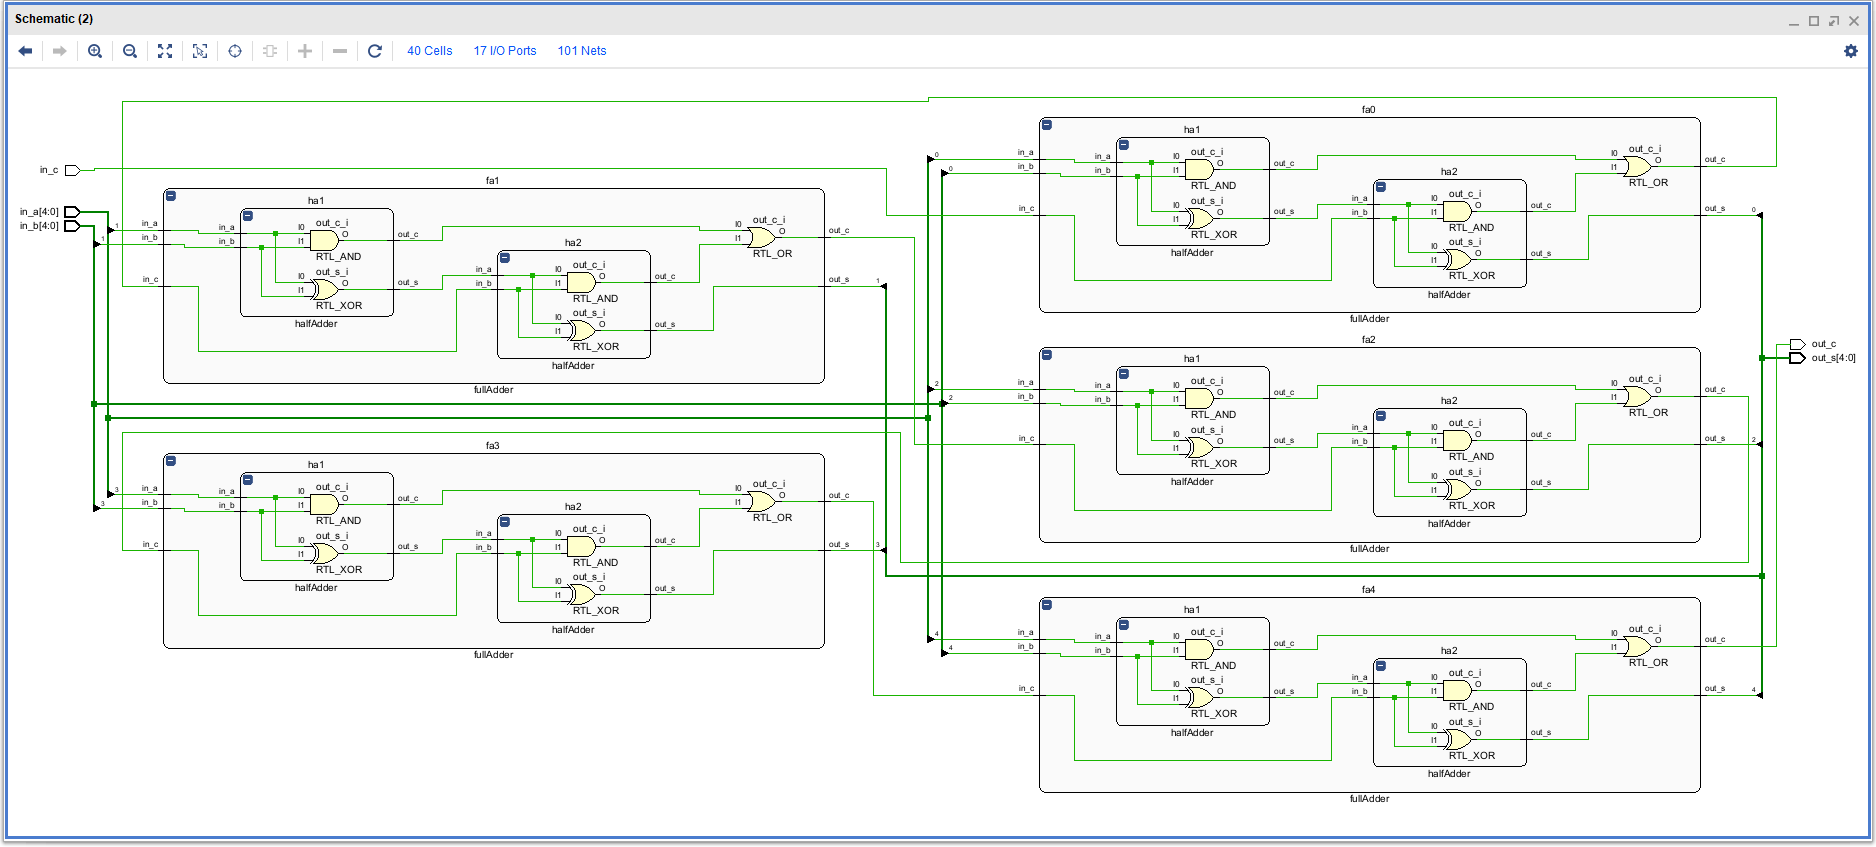
\includegraphics[width=0.9\linewidth]{lab4_2_schematic.png}
\end{figure}
테스트벤치 실행 결과 나온 파형은 다음과 같다.
\begin{figure}[H]
  \centering
  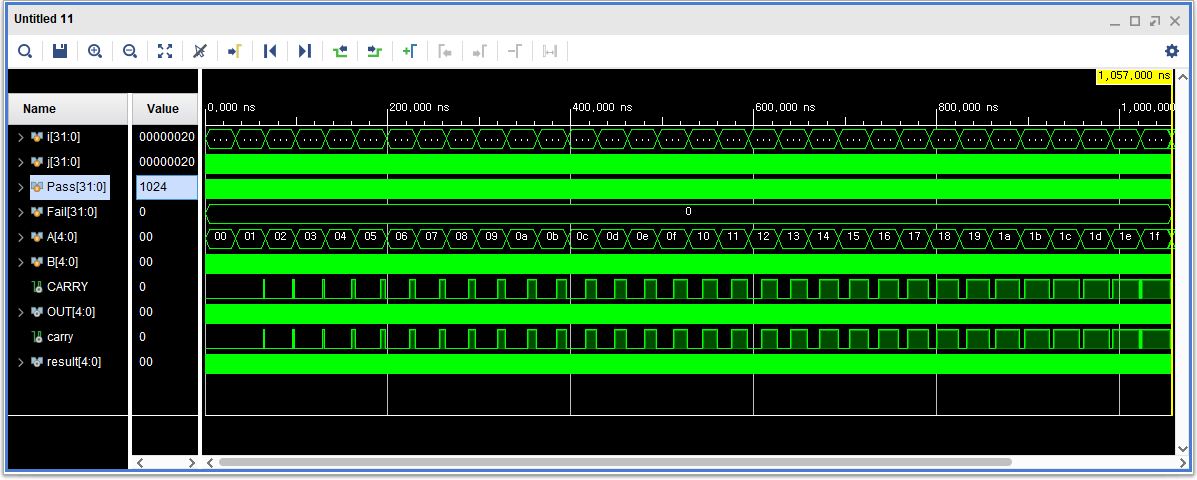
\includegraphics[width=0.9\linewidth]{lab4_2_waveform.png}
\end{figure}

\subsection{\texttt{lab4\_3.v} -- 5-bit 리플 감산기}
회로도는 다음과 같다.
\begin{figure}[H]
  \centering
  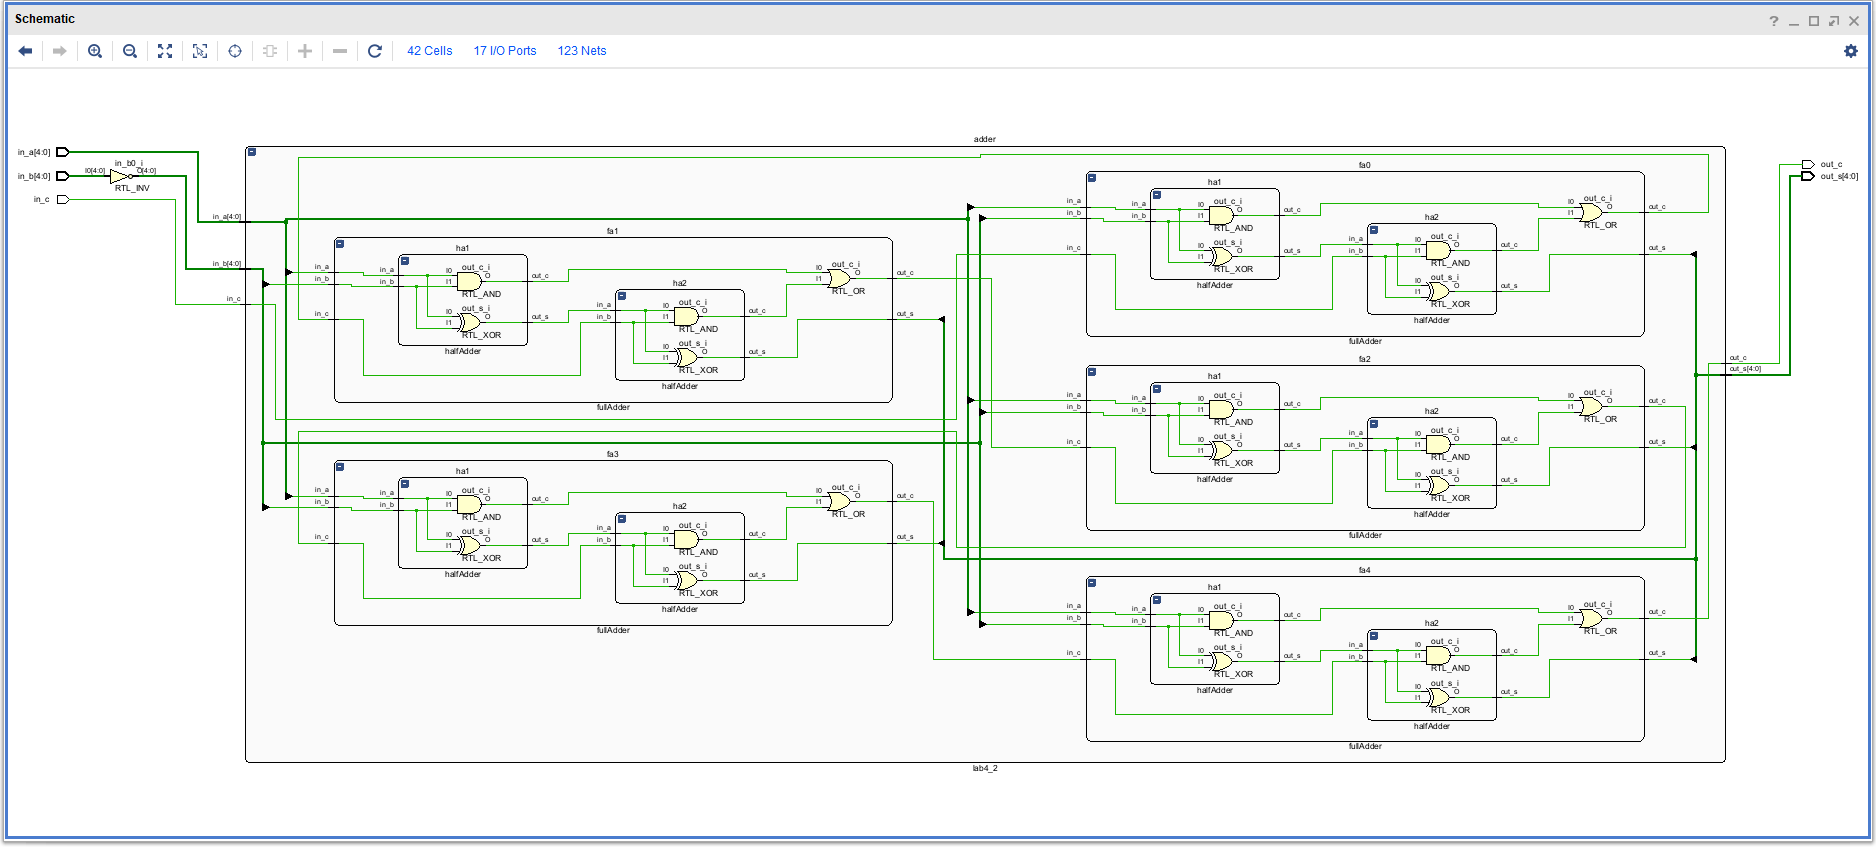
\includegraphics[width=0.9\linewidth]{lab4_3_schematic.png}
\end{figure}
테스트벤치 실행 결과 나온 파형은 다음과 같다.
\begin{figure}[H]
  \centering
  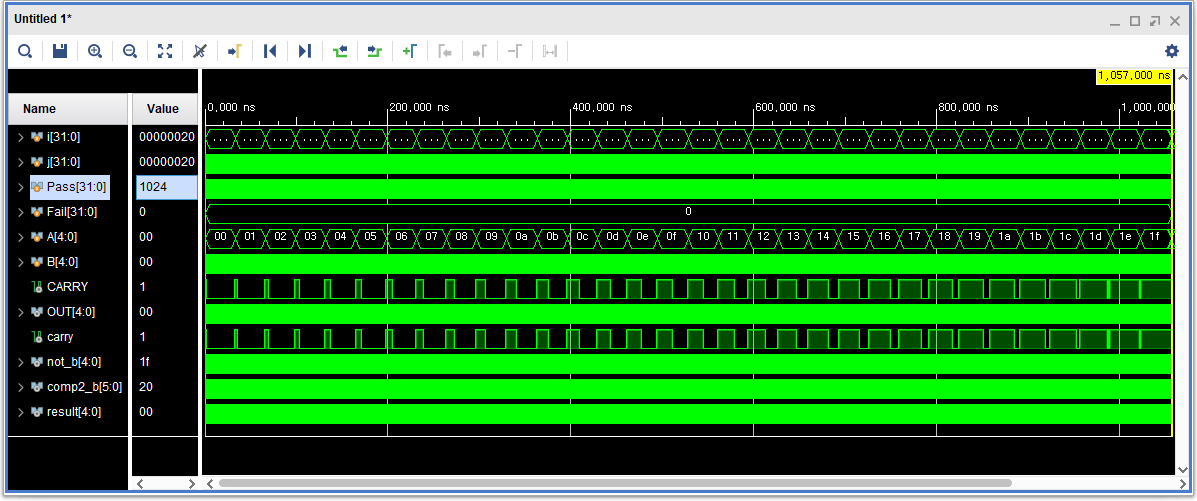
\includegraphics[width=0.9\linewidth]{lab4_3_waveform.png}
\end{figure}

\subsection{\texttt{lab4\_4.v} -- 5-by-3 이진 곱셈기}
회로도는 다음과 같다.
\begin{figure}[H]
  \centering
  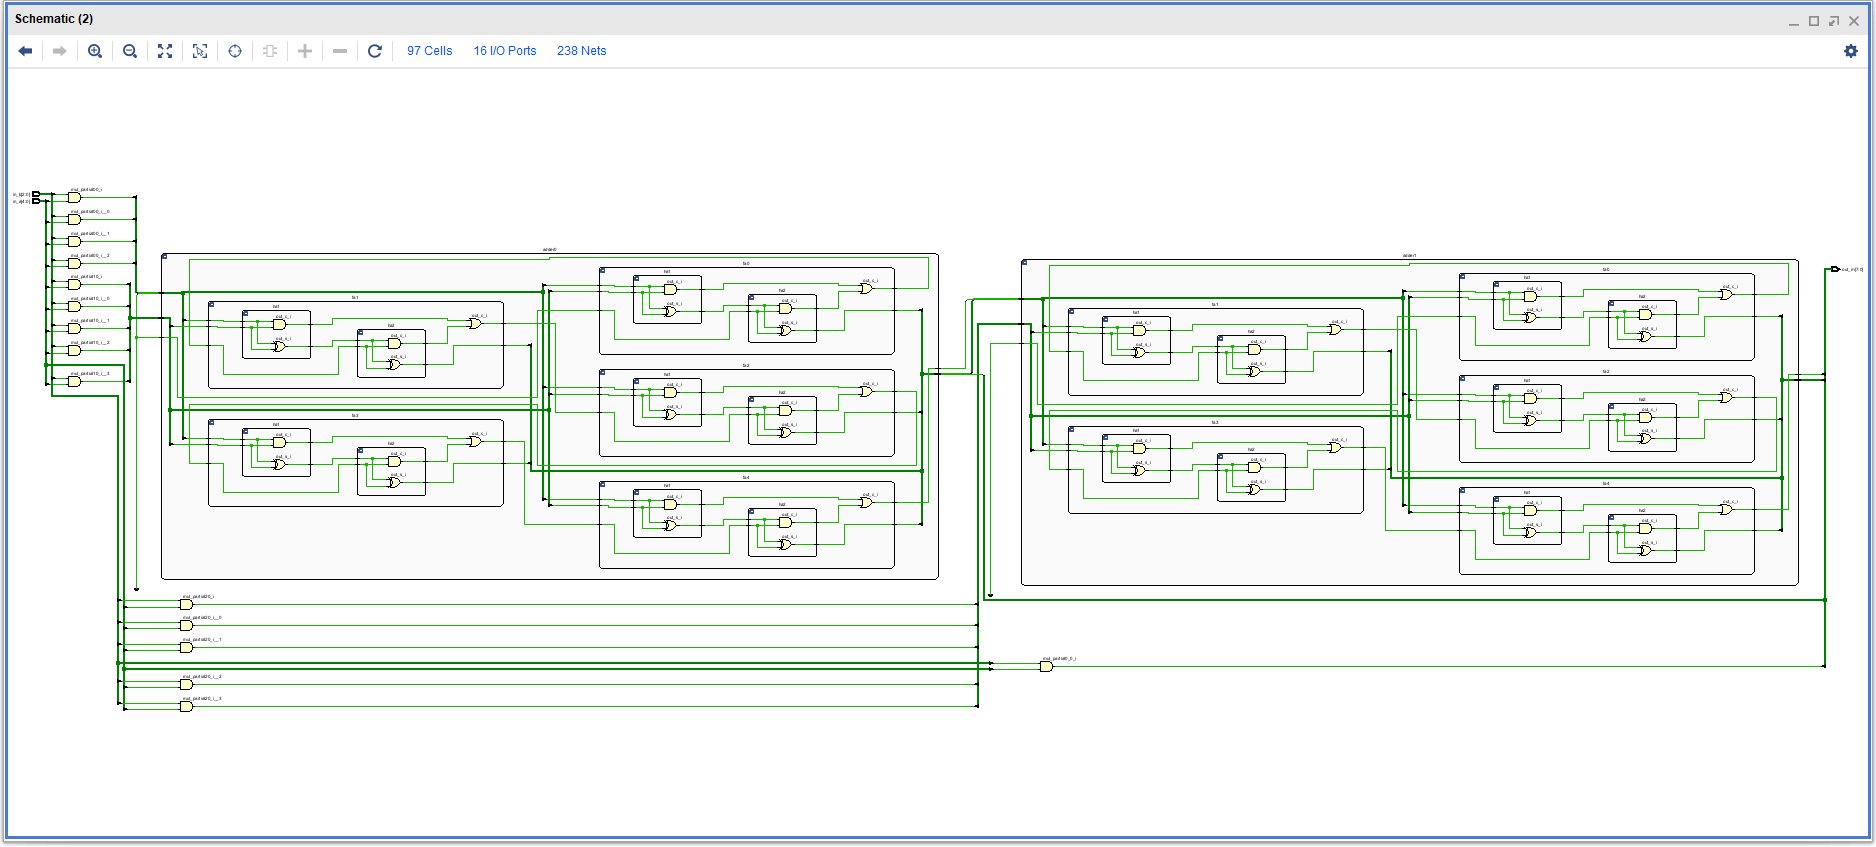
\includegraphics[width=0.9\linewidth]{lab4_4_schematic.png}
\end{figure}
테스트벤치 실행 결과 나온 파형은 다음과 같다.
\begin{figure}[H]
  \centering
  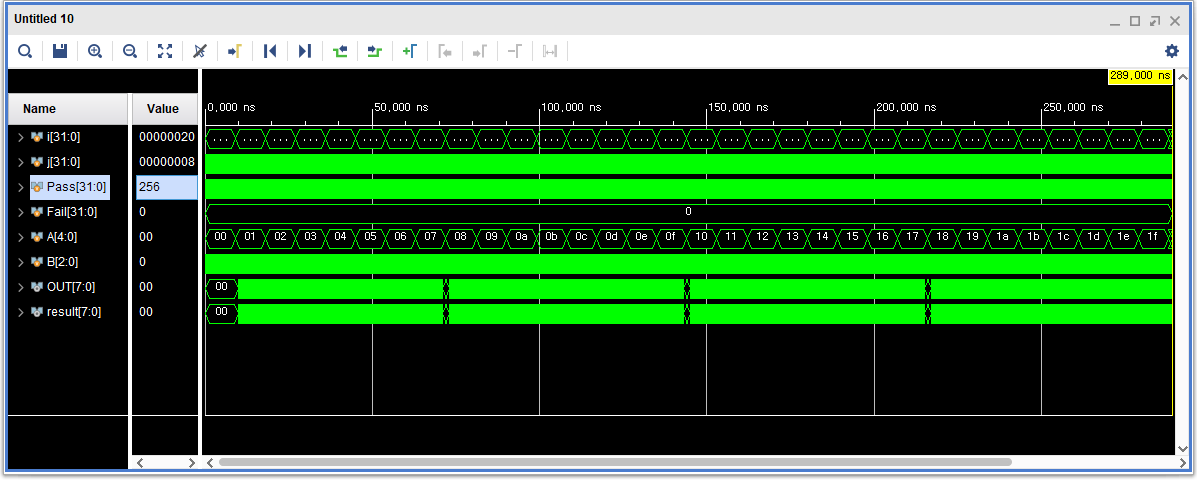
\includegraphics[width=0.9\linewidth]{lab4_4_waveform.png}
\end{figure}

\section{논의}
\end{document}
